\documentclass[letterpaper,12pt]{article}
\usepackage{epsfig,latexsym,amsmath,amssymb,epic,eepic,psfrag,subfigure,float,euscript,array}
\usepackage[latin1]{inputenc}
\usepackage{standalone}
\usepackage{tikz,pgf,pgfplots}
\usepackage[margin=2.5cm]{geometry}
\usepackage[amssymb]{SIunits}

\newenvironment{exercise}[1][Uppgift]{\begin{trivlist} \item[\hskip
    \labelsep {\stepcounter{exerctr}\bfseries #1
      \arabic{exerctr}}]}{\end{trivlist}\vspace{10mm}}

\newcounter{exerctr}
\newcounter{abcctr}[exerctr]

\newcommand{\abc}{\noindent\vspace{1mm}\\ {\bf
    \stepcounter{abcctr}(\alph{abcctr})\ }}
\newcommand{\bbm}{\begin{bmatrix}}
\newcommand{\ebm}{\end{bmatrix}}
\newcommand{\point}[1]{\hfill {\bf (#1p)}\\ \vspace{-5mm}}
\newcommand{\ctrb}{\EuScript{S}}
\newcommand{\Lap}{\mathcal{L}}
\newcommand{\obsv}{\EuScript{O}}
\newcommand{\realdel}[1]{\text{Re}\left\{#1\right\}}
\newcommand{\imagdel}{\text{Im}}
\newcommand{\bC}{\mathbb{C}}
\newcommand{\bR}{\mathbb{R}}
\newcommand{\bmpv}{\begin{minipage}[t]}
\newcommand{\bmps}{\begin{minipage}[t]{45mm}}
\newcommand{\bmpm}{\begin{minipage}[t]{90mm}}
\newcommand{\bmpl}{\begin{minipage}[t]{\textwidth}}
\newcommand{\emp}{\end{minipage}}
\newcommand*{\zethree}{\big(z - \mexp{-3h}\big)}
\newcommand*{\mexp}[1]{\ensuremath{\mathrm{e}^{#1}}}

\newcommand*\circled[1]{\tikz[baseline=(char.base)]{
            \node[shape=circle,draw,inner sep=2pt] (char) {#1};}}

\addtolength{\topmargin}{-1cm}
\textheight 23.5cm
%\oddsidemargin 0.61cm
%\evensidemargin 0.61cm


\def\OctaveG{tf([0.5 1], [1 0 -1])}

\title{Computerized control partial exam 2 (15\%)}
\author{Kjartan Halvorsen}

\begin{document}

\maketitle


\begin{description}
\item[Time] 2017-03-28 17:35 - 19:00
\item[Place] 5105
\item[Permitted aids] The single colored page with your own notes, table of Laplace transforms, calculator
\end{description}

All answers should be readable and well motivated (if nothing else is written). Solutions/motivations should be written on the provided spaces in this exam. Use the last page if more space is needed.

\begin{center}
{\Large Good luck!} \\
\end{center}

\noindent
\fbox{
\bmpl
{\bf Matricual and name:}\\
\vspace*{30mm}
\emp}

\clearpage

%-----------------------------------------------------------------


\subsection*{Problem 1 (60p)}
%----------------------
% RST design for sampled harmonic oscillator
%----------------------


\subsubsection*{(a) 40p}
The plant to be controlled in figure \ref{fig:2dof} is a harmonic oscillator with resonance frequency \unit{1}{\rad\per\second}.  In continuous-time it is described by the transfer function
\begin{equation}
G(s) = \frac{\omega_0^2}{s^2 + \omega_0^2}, \quad \omega_0 = 1.
\end{equation}
Zero-order-hold sampling gives the discrete-time model
\begin{equation}
H(z) = \frac{(1-\beta)(z+1)}{z^2 -2\beta z + 1}, \quad \beta = \cos( \omega_0 h).
\end{equation}
Use the value $\omega_0 h = 0.35$ which gives $\beta \approx 0.94$. 
 
The following specifications on the closed-loop system are given:
\begin{itemize}
\item The closed loop system from the command signal to the output should have the characteristic polynomial
  \begin{equation}
    A_c(z) = (z-0.4)^2
  \end{equation}
  and unit static gain \(H_c(1) = \frac{B_c(1)}{A_c(1)} = 1\).
\item  All observer poles should be placed in the origin.
\item The controller polynomials should have as low degree as possible.
\end{itemize}

Determine the polynomials \(R(z)\), \(S(z)\) and \(T(z)\) in an RST-controller of the form in figure~\ref{fig:2dof}, such that the specifications are satisfied. You can assume the problem to be solved once you have determined $T(z)$ and have written up the correct linear equations in the unknown controller parameters of $R(z)$ and $S(z)$. You don't have to solve this system of equations. Hint: $R(z) = z + 0.495$. 

\begin{figure}
\begin{center}
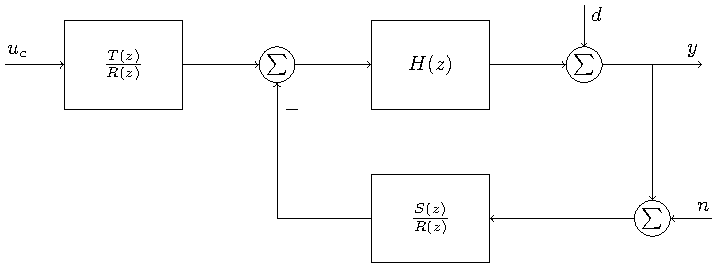
\includegraphics[width=0.7\linewidth]{../../homework/rst-block}
\caption{RST controller}
\label{fig:2dof}
\end{center}
\end{figure}

\noindent
\fbox{
\bmpl
{\bf Controller design:}\\
\vspace*{250mm}
%\vfill
\emp}



\subsubsection*{(b) 20p}

Determine the closed-loop pulse transfer function $H_{d}(z)$ from the disturbance $d$ to the output $y$, and calculate the steady-state error for constant disturbances, i.e.~calculate $\lim_{k\to\infty} y(k)$ for input signals $u_c=0$ and $d = 1$. Use $R(z) = z + 0.495$. 

\noindent
\fbox{
\bmpl
{\bf Solution:}\\
\vspace*{120mm}
\emp}


%\clearpage
\subsection*{Problem 2 (40p)}
Instead of the 2-degrees-of-freedom structure of figure \ref{fig:2dof}, consider now that the harmonic oscillator is controlled using feedback from the error signal as in figure \ref{fig:feedback}. 
\begin{figure}[b]
\begin{center}
     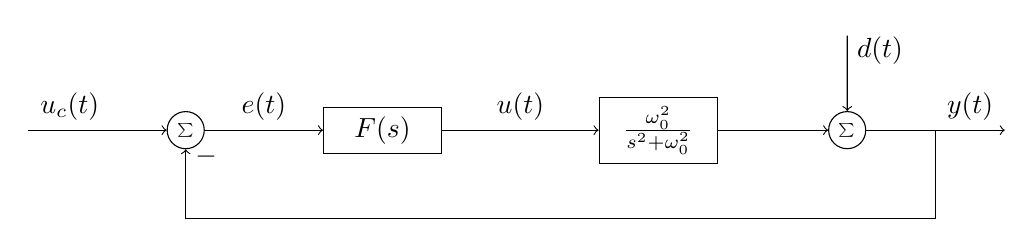
\begin{tikzpicture}[scale = 0.8, node distance=25mm, block/.style={rectangle, draw, minimum width=15mm}, sumnode/.style={circle, draw, inner sep=2pt}]
     
     \node[coordinate] (refinput) {};
     \node[sumnode, right of=refinput, node distance=20mm] (sumerr) {\tiny $\sum$};
     \node[block, right of=sumerr] (controller) {$F(s)$};
     %\node[above of=controller, node distance=6mm] {controller};
     \node[block, right of=controller, node distance=35mm] (plant) {$\frac{\omega_0^2}{s^2 + \omega_0^2}$};
     \node[sumnode, right of=plant, node distance=24mm] (sum) {\tiny $\sum$};
     %\node[above of=tank, node distance=6mm] {motor};
     \node[coordinate, right of=sum, node distance=20mm] (output) {};
     \node[coordinate, above of=sum, node distance=12mm] (disturbance) {};

     \draw[->] (refinput) -- node[above, pos=0.3] {$u_c(t)$} (sumerr);
     \draw[->] (sumerr) -- node[above] {$e(t)$} (controller);
     \draw[->] (controller) -- node[above] {$u(t)$} (plant);
     \draw[->] (plant) -- (sum);
     \draw[->] (sum) -- node [coordinate] (measure)  {} node [above, near end] {$y(t)$} (output);
     \draw[->] (disturbance) -- node[right, pos=0.2] {$d(t)$} (sum);
     \draw[->] (measure) -- ++(0,-14mm) -| node[right, pos=0.95] {$-$} (sumerr);
     \end{tikzpicture}
     \caption{Feedback control from the error signal.}
     \label{fig:feedback}
   \end{center}
 \end{figure}

A lead-lag compensator has been designed in continuous-time. It has the transfer function
\begin{equation}
F(s) = \frac{15s + 3}{s + 7} \cdot \frac{1.5s + 1}{1.5s}
\end{equation}
 
\subsubsection*{(a) 20p}
Discretize the controller $F(s)$ using Tustin's approximation
\[ s = \frac{2}{h}\cdot\frac{z-1}{z+1} \]
and determine the poles and zeros of the discrete-time controller. Use the same sampling period $h=0.35$ as in the previous problem.

\noindent
\fbox{
\bmpl
{\bf Solution:}\\
\vspace*{170mm}
\emp}


\subsubsection*{(b) 10p}
Figure \ref{fig:sim} shows responses of the closed-loop systems obtained with the RST-controller and with the discretized lead-lag-controller, respectively.  Which response corresponds to which controller? Motivate your answer!


\noindent
\fbox{
\bmpl
{\bf Answer and motivation:}\\
\vspace*{80mm}
\emp}

\begin{figure}[hb]
\begin{center}
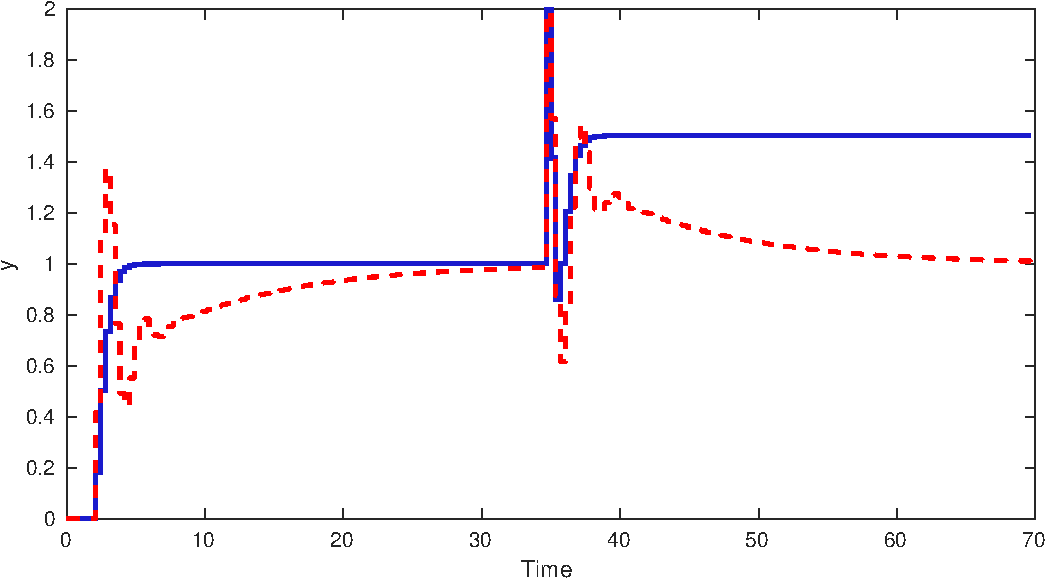
\includegraphics[width=0.9\linewidth]{RST_leadlag_sim-crop}
\caption{Response of the closed-loop system obtained with an RST controller and with a discretized lead-lag controller. At time $t=5h$ a step in the command signal $u_c(kh)$ occurs, and at $t=100h$ a step in the disturbance signal $d(kh)$ occurs. }
\label{fig:sim}
\end{center}
\end{figure}



\subsubsection*{(c) 10p}
Study figure \ref{fig:sim} and write down \textbf{three} relevant observations about the behaviour of the closed-loop systems. Suggest an improvement to the RST controller. 

\noindent
\fbox{ 
\bmpl
{\bf Answer:}\\
\vspace*{100mm}
\emp}


\cleardoublepage

\noindent
{\bf If necessary,} you can continue your solutions on this sheet. Mark clearly which problem the solution corresponds to.

%\end{document}

\section*{Solutions}
\subsection*{Problem 1}

\subsubsection*{(a)}
This problem is quite straightforward RST design. There are no requirement that constant distubances on the output must be eliminated, and so we do not need to include an integrator in the feedback controller. The Diophantine equation is 
\begin{align*}
A(z) R(z) + B(z) S(z) &= A_c(z)A_o(z).
\end{align*}
The order of the controller should be as low as possible, while still giving us sufficient flexibility to obtain the desired second order polynomial $A_c(z)=(z-0.4)^2 = z^2 - 0.8z + 0.16$. Since the polynomial $A(z)$ is of degree two, we have that the Diophantine equation will be of degree $n_R + 2$, and will give as many equations in the unknowns when we set the coefficients on both sides of the equality sign equal. 

The controller is \(\frac{S(z)}{R(z)}\) which has \(2n_R + 1\) unknown coefficients when $S(z)$ and $R(z)$ are of the same degree. These coefficients are to be determined from the Diophantine equation, so we must have
\[ 2n_R + 1 = n_R + 2 \quad \Rightarrow \quad n_R = 1. \]
The left hand side of the Diophantine equation is of degree 3, so then we need a single observer pole in the origin, $A_o(z)=z$. 
We can now set up the Diophantine equation
\[ (z^2 - 1.879z + 1)(z+r_1) + 0.061(z + 1)(s_0z + s_1) = (z^2 - 0.8z + 0.16)z\]
or
\[ z^3 + (r_1 + 0.061s_0 - 1.879)z^2 + (- 1.879r_1 + 0.061s_0 + 0.061s_1 + 1)z + r_1 + 0.061s_1 = z^3 - 0.8z^2 + 0.16z,\]  
from which we get
\begin{align*}
 r_1 + 0.061s_0 &= -0.8+1.879\\
-1.879r_1 + 0.061s_0 + 0.061s_1 &= 0.16-1\\
r_1 + 0.061s_1 &= 0.
\end{align*}
This is sufficient solution for this part of the exercise. Actually solving the system of equations gives
\begin{align*}
r_1 &= 0.495\\
s_0 &= 9.63\\
s_1 &= -8.16
\end{align*}

With $T(z) = t_0 A_0(z)$, the closed-loop system becomes
\[ H_c(z) = \frac{T(z)B(z)}{A(z)R(z) + B(z)S(z)} =   \frac{t_0B(z)}{A_c(z)}. \]
Unit static gain is obtained with 
\[ t_0 = \frac{A_c(1)}{B(1)} = \frac{0.36}{0.121} = 2.97. \]

The controller is thus
\begin{align*}
H_{fb}(z) &= \frac{S(z)}{R(z)} = \frac{9.63z - 8.16}{z + 0.495}\\
H_{ff}(z) &= \frac{T(z)}{R(z)} = \frac{2.97z}{z + 0.495}. 
\end{align*}

\subsubsection*{(b)}
Using Mason's rule:
\begin{equation*}
\begin{split}
 H_d(z) &= \frac{1}{1 + \frac{B}{A}\cdot\frac{S}{R}} = \frac{A(z)R(z)}{A(z)R(z) + B(z)S(z)} \\
        &= \frac{A(z)R(z)}{A_c(z)A_o(z)} = \frac{(z^2 - 1.879z + 1)(z + 0.495)}{(z-0.4)^2z},
      \end{split}
\end{equation*}
which has static gain
\[ H_d(1) = \frac{(1 - 1.879 + 1)(1.495)}{0.36} = 0.503.\]
so
\begin{equation*}
\begin{split}
\lim_{k\to\infty} y(k) &= \lim_{z\to 1} (z-1) Y(z) = \lim_{z\to 1} (z-1) H_d(z) \frac{z}{z-1}\\
 &= H_d(1) = 0.503. 
\end{split}
\end{equation*}

\subsection*{Problem 2}

\subsubsection*{(a)}

Inserting the expression for Tustin's approximation we get
\begin{equation*}
\begin{split}
F_d(z) &= F(s)|_{s = \frac{2}{h}\cdot\frac{z-1}{z+1}} \\
 &= \frac{ 15 \frac{2}{h}\cdot\frac{z-1}{z+1} + 3}{ \frac{2}{h}\cdot\frac{z-1}{z+1} + 7 } \cdot \frac{1.5\frac{2}{h}\cdot\frac{z-1}{z+1} + 1}{ 1.5\frac{2}{h}\cdot\frac{z-1}{z+1} } \\
&= \frac{\big(30(z-1) + 3\cdot 0.35(z+1)\big) \big( 3(z-1) + 0.35(z+1)\big)}{\big(2(z-1) + 7\cdot 0.35(z+1)\big)3(z-1)}\\
&= \frac{(31.05z -28.95)(3.35z - 2.65)}{3(4.45z + 0.45)(z-1)}.
\end{split}
\end{equation*}
There are two poles
\[ z = -\frac{0.45}{4.45} \approx -0.101 \quad \text{and} \quad z = 1\]
and two zeros
\[ z = \frac{28.95}{31.05} \approx 0.93 \quad \text{and} \quad z = \frac{2.65}{3.35} \approx 0.79. \]

\subsubsection*{(b)}

It is probably easiest to see the difference in the response to the disturbance at $t=100h$. The solid line has a stationary error, but the dashed has not. The RST controller has no integrator but the lead-lag compensator does. The integrator in the lead-lag compensator eliminates the constant disturbance. So, the solid line corresponds to the response of the RST controlled system, and the dashed line corresponds to the system controlled with a lead-lag compensator.
 
It can also be seen from the fact that the designed closed-loop system of the RST controller has real-valued poles. Such a system should not give the high overshoot of the dashed line. 

\subsubsection*{(c)}

Suggested observations:
\begin{itemize}
\item The dashed line has significant overshoot. This suggests a small phase margin.
\item The solid line has no overshoot. This suggests real-valued poles.
\item The dashed line goes more slowly to the final value. This suggests the existence of a slow pole close to the origin.  
\item The dashed line eliminates the constant disturbance, so the loop gain has infinite static gain, i.e.~it contains an integrator.
\item The solid line shows a persisting error when a disturbance is present. 
\end{itemize}


The only real problem with the response of the RST controller is that the disturbance is not eliminated. We could fix this by introducing an integrator in the RST controller (incremental RST), i.e.~set
\[ R(z) = (z-1)\bar{R}(z)\]
and redo the design.
\end{document}
